%-------------------------------------------------------------------------------
%                            BAB III
%               		METODOLOGI PENELITIAN
%-------------------------------------------------------------------------------
% \fancyhf{} 
% \fancyfoot[R]{\thepage}
\chapter{METODE PENENILITIAN}
%\thispagestyle{plain} % Halaman pertama bab menggunakan gaya plain
\section{Deskripsi Lokasi Penelitian}
Lokasi kampus II USK terdiri dari 4 kecamatan (Baitussalam, Mesjid Raya, 
Darussalam, Kuta Baro), namun penelitian ini hanya memfokuskan pada Kecamatan 
Mesjid raya yang merupakan bagian tanah Kampus II USK sesuai dengan prioritas
kebutuhan tanah untuk lokasi pengembangan kampus seluas 250 Ha, Gambar \ref{batas dan area studi} menunjukan batas tanah Kampus II USK dan area studi penelitian.

\begin{figure}[H]
\centering
\frame{\includegraphics [width = 9cm]{image/Tanah Kampus II USK}}
\caption{Batas tanah kampus II USK seluas 1.588 Ha (kuning), dan batas area studi penelitian seluas 250 Ha (biru)
}
\label{batas dan area studi}
\end{figure}

\section{Waktu dan Lokasi Penelitian}
Penelitian ini dilaksanakan mulai dari bulan Maret hingga Agustus 2024, melibatkan serangkaian aktivitas di laboratorium. Kegiatan laboratorium melibatkan proses pengolahan citra, yang dilakukan di Laboratorium Terpadu Sistem Informasi Geografis dan Data Spasial USK. Rincian jadwal penelitian dapat dilihat pada Tabel 3.1 berikut.

% Please add the following required packages to your document preamble:
% \usepackage{multirow}
% \usepackage[table,xcdraw]{xcolor}
% Beamer presentation requires \usepackage{colortbl} instead of \usepackage[table,xcdraw]{xcolor}
\begin{table}[H]
  \caption{Distribusi Jadwal Kegiatan Penelitian Bulan Maret-Agustus 2024}
  \label{tab:jadwal-kegiatan-januari-maret-2024}
  \resizebox{\columnwidth}{!}{%
  \begin{tabular}{|c|l|llll|llll|llll|llll|llll|llll|}
  \hline
                       & \multicolumn{1}{c|}{}                           & \multicolumn{4}{c|}{Maret}                                                                                                                                             & \multicolumn{4}{c|}{April}                                                                                                                                            & \multicolumn{4}{c|}{Mei}                                                                                                                                               & \multicolumn{4}{c|}{Juni}                                                                                                                                                                                             & \multicolumn{4}{c|}{Juli}                                                                                                                                                 & \multicolumn{4}{c|}{Agustus}                                                                                                                                                \\ \cline{3-26} 
                       & \multicolumn{1}{c|}{}                           & \multicolumn{4}{c|}{Minggu Ke-}                                                                                                                                          & \multicolumn{4}{c|}{Minggu Ke-}                                                                                                                                          & \multicolumn{4}{c|}{Minggu Ke-}                                                                                                                                          & \multicolumn{4}{c|}{Minggu Ke-}                                                                                                                                                                                        & \multicolumn{4}{c|}{Minggu Ke-}                                                                                                                                          & \multicolumn{4}{c|}{Minggu Ke-}                                                                                                                                          \\ \cline{3-26} 
  \multirow{-3}{*}{No} & \multicolumn{1}{c|}{\multirow{-3}{*}{Kegiatan}} & \multicolumn{1}{c|}{1}                        & \multicolumn{1}{c|}{2}                        & \multicolumn{1}{c|}{3}                        & \multicolumn{1}{c|}{4}   & \multicolumn{1}{c|}{1}                        & \multicolumn{1}{c|}{2}                        & \multicolumn{1}{c|}{3}                        & \multicolumn{1}{c|}{4}   & \multicolumn{1}{c|}{1}                        & \multicolumn{1}{c|}{2}                        & \multicolumn{1}{c|}{3}                        & \multicolumn{1}{c|}{4}   & \multicolumn{1}{c|}{1}                                               & \multicolumn{1}{c|}{2}                                               & \multicolumn{1}{c|}{3}                        & \multicolumn{1}{c|}{4}   & \multicolumn{1}{c|}{1}                        & \multicolumn{1}{c|}{2}                        & \multicolumn{1}{c|}{3}                        & \multicolumn{1}{c|}{4}   & \multicolumn{1}{c|}{1}                        & \multicolumn{1}{c|}{2}                        & \multicolumn{1}{c|}{3}                        & \multicolumn{1}{c|}{4}   \\ \hline
  
  1                    & Studi Literatur                                 & \multicolumn{1}{l|}{\cellcolor[HTML]{656565}} & \multicolumn{1}{l|}{\cellcolor[HTML]{656565}} & \multicolumn{1}{l|}{\cellcolor[HTML]{656565}} & \cellcolor[HTML]{656565} & \multicolumn{1}{l|}{\cellcolor[HTML]{656565}} & \multicolumn{1}{l|}{\cellcolor[HTML]{656565}} & \multicolumn{1}{l|}{\cellcolor[HTML]{656565}} & \cellcolor[HTML]{656565} & \multicolumn{1}{l|}{\cellcolor[HTML]{656565}} & \multicolumn{1}{l|}{\cellcolor[HTML]{656565}} & \multicolumn{1}{l|}{\cellcolor[HTML]{656565}} & \cellcolor[HTML]{656565} & \multicolumn{1}{l|}{}                                                & \multicolumn{1}{l|}{}                                                & \multicolumn{1}{l|}{}                         &                          & \multicolumn{1}{l|}{}                         & \multicolumn{1}{l|}{}                         & \multicolumn{1}{l|}{}                         &                          & \multicolumn{1}{l|}{}                         & \multicolumn{1}{l|}{}                         & \multicolumn{1}{l|}{}                         &                          \\ \hline
  2                    & Analisis Akuisisi Data                                & \multicolumn{1}{l|}{}                         & \multicolumn{1}{l|}{}                         & \multicolumn{1}{l|}{}                         & & \multicolumn{1}{l|}{\cellcolor[HTML]{656565}} & \multicolumn{1}{l|}{\cellcolor[HTML]{656565}}                         & \multicolumn{1}{l|}{\cellcolor[HTML]{656565}}                         &                          \cellcolor[HTML]{656565}& \multicolumn{1}{l|}{\cellcolor[HTML]{656565}} & \multicolumn{1}{l|}{\cellcolor[HTML]{656565}}                         & \multicolumn{1}{l|}{\cellcolor[HTML]{656565}}                         &                          \cellcolor[HTML]{656565}& \multicolumn{1}{l|}{\cellcolor[HTML]{656565}}                                                & \multicolumn{1}{l|}{}                                                & \multicolumn{1}{l|}{}                         &                          & \multicolumn{1}{l|}{}                         & \multicolumn{1}{l|}{}                         & \multicolumn{1}{l|}{}                         &                          & \multicolumn{1}{l|}{}                         & \multicolumn{1}{l|}{}                         & \multicolumn{1}{l|}{}                         &                          \\ \hline
  3                    & Pengumpulan Data                              & \multicolumn{1}{l|}{}                         & \multicolumn{1}{l|}{}                         & \multicolumn{1}{l|}{}                         &                          & \multicolumn{1}{l|}{} & \multicolumn{1}{l|}{} & \multicolumn{1}{l|}{} &                          & \multicolumn{1}{l|}{}                         & \multicolumn{1}{l|}{}                         & \multicolumn{1}{l|}{}                         &                          \cellcolor[HTML]{656565}& \multicolumn{1}{l|}{\cellcolor[HTML]{656565}}                                                & \multicolumn{1}{l|}{\cellcolor[HTML]{656565}}                                                & \multicolumn{1}{l|}{}                         &                          & \multicolumn{1}{l|}{}                         & \multicolumn{1}{l|}{}                         & \multicolumn{1}{l|}{}                         &                          & \multicolumn{1}{l|}{}                         & \multicolumn{1}{l|}{}                         & \multicolumn{1}{l|}{}                         &                          \\ \hline
  4                    & Mosaik Menggunakan Agisoft Metashape                     & \multicolumn{1}{l|}{}                         & \multicolumn{1}{l|}{}                         & \multicolumn{1}{l|}{}                         &                          & \multicolumn{1}{l|}{}                         & \multicolumn{1}{l|}{}                         & \multicolumn{1}{l|}{} & & \multicolumn{1}{l|}{} & \multicolumn{1}{l|}{} & \multicolumn{1}{l|}{} & & \multicolumn{1}{l|}{\cellcolor[HTML]{656565}}                                                & \multicolumn{1}{l|}{\cellcolor[HTML]{656565}}                                                & \multicolumn{1}{l|}{\cellcolor[HTML]{656565}}                         &                          \cellcolor[HTML]{656565}& \multicolumn{1}{l|}{}                         & \multicolumn{1}{l|}{}                         & \multicolumn{1}{l|}{}                         &                          & \multicolumn{1}{l|}{}                         & \multicolumn{1}{l|}{}                         & \multicolumn{1}{l|}{}                         &                          \\ \hline
  5                    & Mosaik Menggunakan PIX4Dmapper                                  & \multicolumn{1}{l|}{}                         & \multicolumn{1}{l|}{}                         & \multicolumn{1}{l|}{}                         &                          & \multicolumn{1}{l|}{}                         & \multicolumn{1}{l|}{}                         & \multicolumn{1}{l|}{}                         &                          & \multicolumn{1}{l|}{}                         & \multicolumn{1}{l|}{}                         & \multicolumn{1}{l|}{}                         &                          & \multicolumn{1}{l|}{} & \multicolumn{1}{l|}{} & \multicolumn{1}{l|}{}                         &                          & \multicolumn{1}{l|}{\cellcolor[HTML]{656565}{\color[HTML]{656565} }}                         & \multicolumn{1}{l|}{\cellcolor[HTML]{656565}{\color[HTML]{656565} }}                         & \multicolumn{1}{l|}{\cellcolor[HTML]{656565}{\color[HTML]{656565} }}                         &                          & \multicolumn{1}{l|}{}                         & \multicolumn{1}{l|}{}                         & \multicolumn{1}{l|}{}                         &                          \\ \hline
  6                    & Analisis Perbandingan Hasil Mosaik                                  & \multicolumn{1}{l|}{}                         & \multicolumn{1}{l|}{}                         & \multicolumn{1}{l|}{}                         &                          & \multicolumn{1}{l|}{}                         & \multicolumn{1}{l|}{}                         & \multicolumn{1}{l|}{}                         &                          & \multicolumn{1}{l|}{}                         & \multicolumn{1}{l|}{}                         & \multicolumn{1}{l|}{}                         &                          & \multicolumn{1}{l|}{}                        & \multicolumn{1}{l|}{}                        & \multicolumn{1}{l|}{} & & \multicolumn{1}{l|}{} & \multicolumn{1}{l|}{} & \multicolumn{1}{l|}{}                         &                          \cellcolor[HTML]{656565}& \multicolumn{1}{l|}{\cellcolor[HTML]{656565}}                         & \multicolumn{1}{l|}{}                         & \multicolumn{1}{l|}{}                         &                          \\ \hline
  7                    & Penyusunan Hasil Penelitian                  & \multicolumn{1}{l|}{}                         & \multicolumn{1}{l|}{}                         & \multicolumn{1}{l|}{}                         &                          & \multicolumn{1}{l|}{}                         & \multicolumn{1}{l|}{}                         & \multicolumn{1}{l|}{}                         &                          & \multicolumn{1}{l|}{}                         & \multicolumn{1}{l|}{}                         & \multicolumn{1}{l|}{}                         &                          & \multicolumn{1}{l|}{}                        & \multicolumn{1}{l|}{}                        & \multicolumn{1}{l|}{} & & \multicolumn{1}{l|}{} & \multicolumn{1}{l|}{} & \multicolumn{1}{l|}{} & & \multicolumn{1}{l|}{\cellcolor[HTML]{656565} }                         & \multicolumn{1}{l|}{\cellcolor[HTML]{656565} }                         & \multicolumn{1}{l|}{\cellcolor[HTML]{656565} }                         &                          \cellcolor[HTML]{656565} \\ \hline
  \end{tabular}%
  }
  \end{table}

\section{Alat dan Bahan}

Alat dan Bahan yang akan digunakan pada penelitian ini terdiri dari beberapa
perangkat keras (\textit{hardware}) dan perangkat lunak (\textit{software}) serta Data Batas administrasi dan foto udara hasil tangkapan \textit{Drone} yang dijabarkan sebagai berikut :

\subsection{Perangkat Keras}

Perangkat keras digunakan sebagai komponen fisik yang mendukung atau menjalankan penelitian. Dalam konteks ini, perangkat keras yang digunakan adalah :

\begin{itemize}
	\item PC Desktop Rakitan dengan CPU Intel® Core™ i5-11500 Processor (12M Cache, up to 4.60 GHz), VGA Nvidia GeForce RTX 2060 SUPER™ 8GB GDDR6, RAM 16GB DDR4 3200Mhz, Penyimpanan SSD 1TB dan HDD 1TB.
    \item Drone DJI Phantom 4 Pro dengan spesifikasi 1" 20MP CMOS Sensor, Gimbal-\textit{Stabilized} 4K60 / 20MP \textit{Imaging, Ocusync Transmission, FlightAutonomy with Redundant Sensors, Four Directions of Obstacle Avoidance, Top Speed of} 45 mph \textit{in Sport Mode, Maximum Control Range of} 4.3 \textit{Miles}, \textit{Visual Tracking of Moving Subject, Up to} 30 \textit{Minutes Flying Time}.
    \item  GPS Geodetic GNSS RTK dari Hi-Target.
	\end{itemize}

\subsection{Perangkat Lunak}

Perangkat lunak merupakan aplikasi atau program yang digunakan untuk mendukung atau melaksanakan penelitian. Dalam penelitian ini, perangkat lunak yang digunakan adalah :

\begin{itemize}
	\item Agisoft Metashape 2.1.1
    \item PIX4Dmapper 4.5.6
    \item ArcGIS 10.8
    \item Google Chrome
    \item DroneDeploy
    \item Google Earth Pro 7.3.6
	\end{itemize}

\subsection{Data}

Data yang digunakan dalam penelitian ini terdiri dari data teks dan data gambar, data teks berupa data koordinat vertikal, horizontal dan ketinggian yang diambil menggunakan GPS Geodetic. sedangkan data gambar berupa serangkaian citra foto udara yang diambil menggunakan \textit{drone} di lahan kampus II Universitas Syiah Kuala. Luas keseluruhan area yang dicakup adalah 250 hektar, dengan jumlah citra mencapai 4701. data juga mencakup batas administrasi lahan kampus II Universitas Syiah Kuala seluas 1588 hektar dan area studi penelitian yang berukuran 250 hektar. Berikut kumpulan dan 3 sampel citra udara hasil tangkapan \textit{drone} seperti yang terlihat pada gambar \ref{citra udara}, \ref{Sampel foto Udara 1}, \ref{Sampel foto Udara 2}, dan \ref{Sampel foto Udara 3}.

\begin{figure}[H]
	\centering
	\frame{\includegraphics [width = 11.5cm,]{image/Kumpulan Citra}}
	\caption{Kumpulan citra udara yang digunakan dalam penelitian ini}
	\label{citra udara} % cuman gambar dummy ya !
\end{figure}

\begin{figure}[H]
        \centering
	\frame{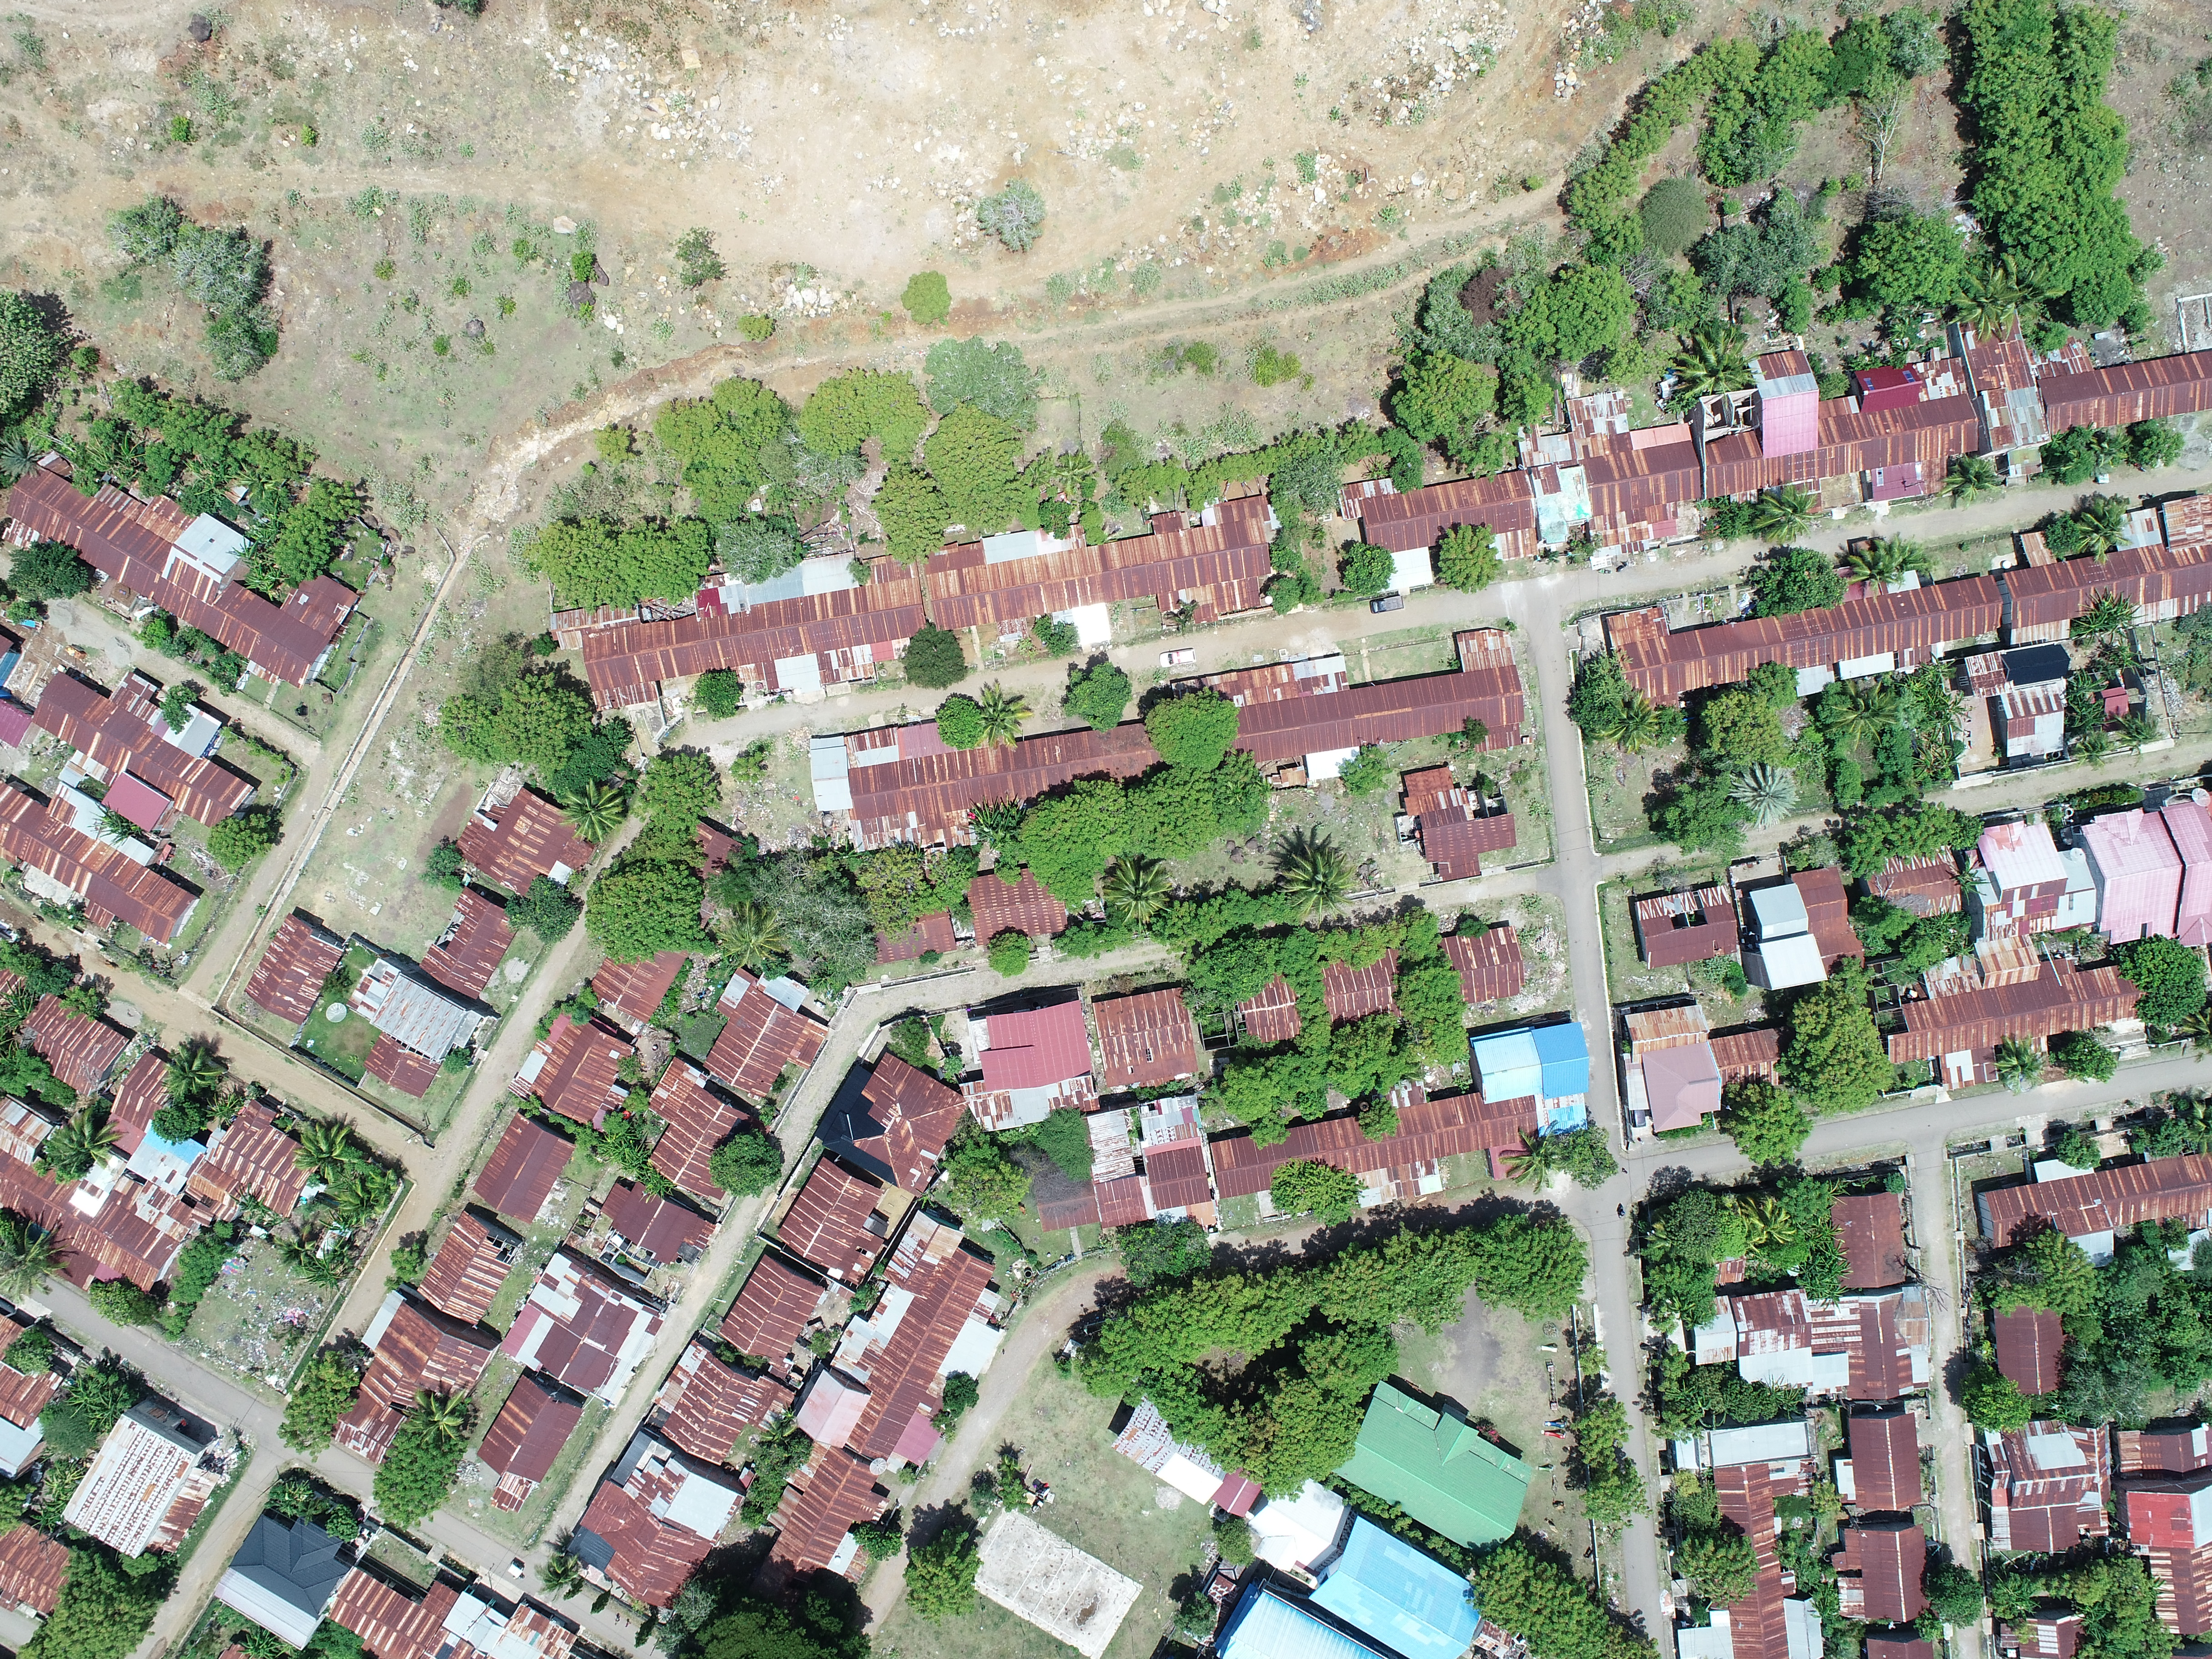
\includegraphics [width = 11.5cm,]{image/DJI_0879}}
	\caption{Sampel foto Udara 1}
	\label{Sampel foto Udara 1} % cuman gambar dummy ya !
\end{figure}
\begin{figure}[H]
        \centering
	\frame{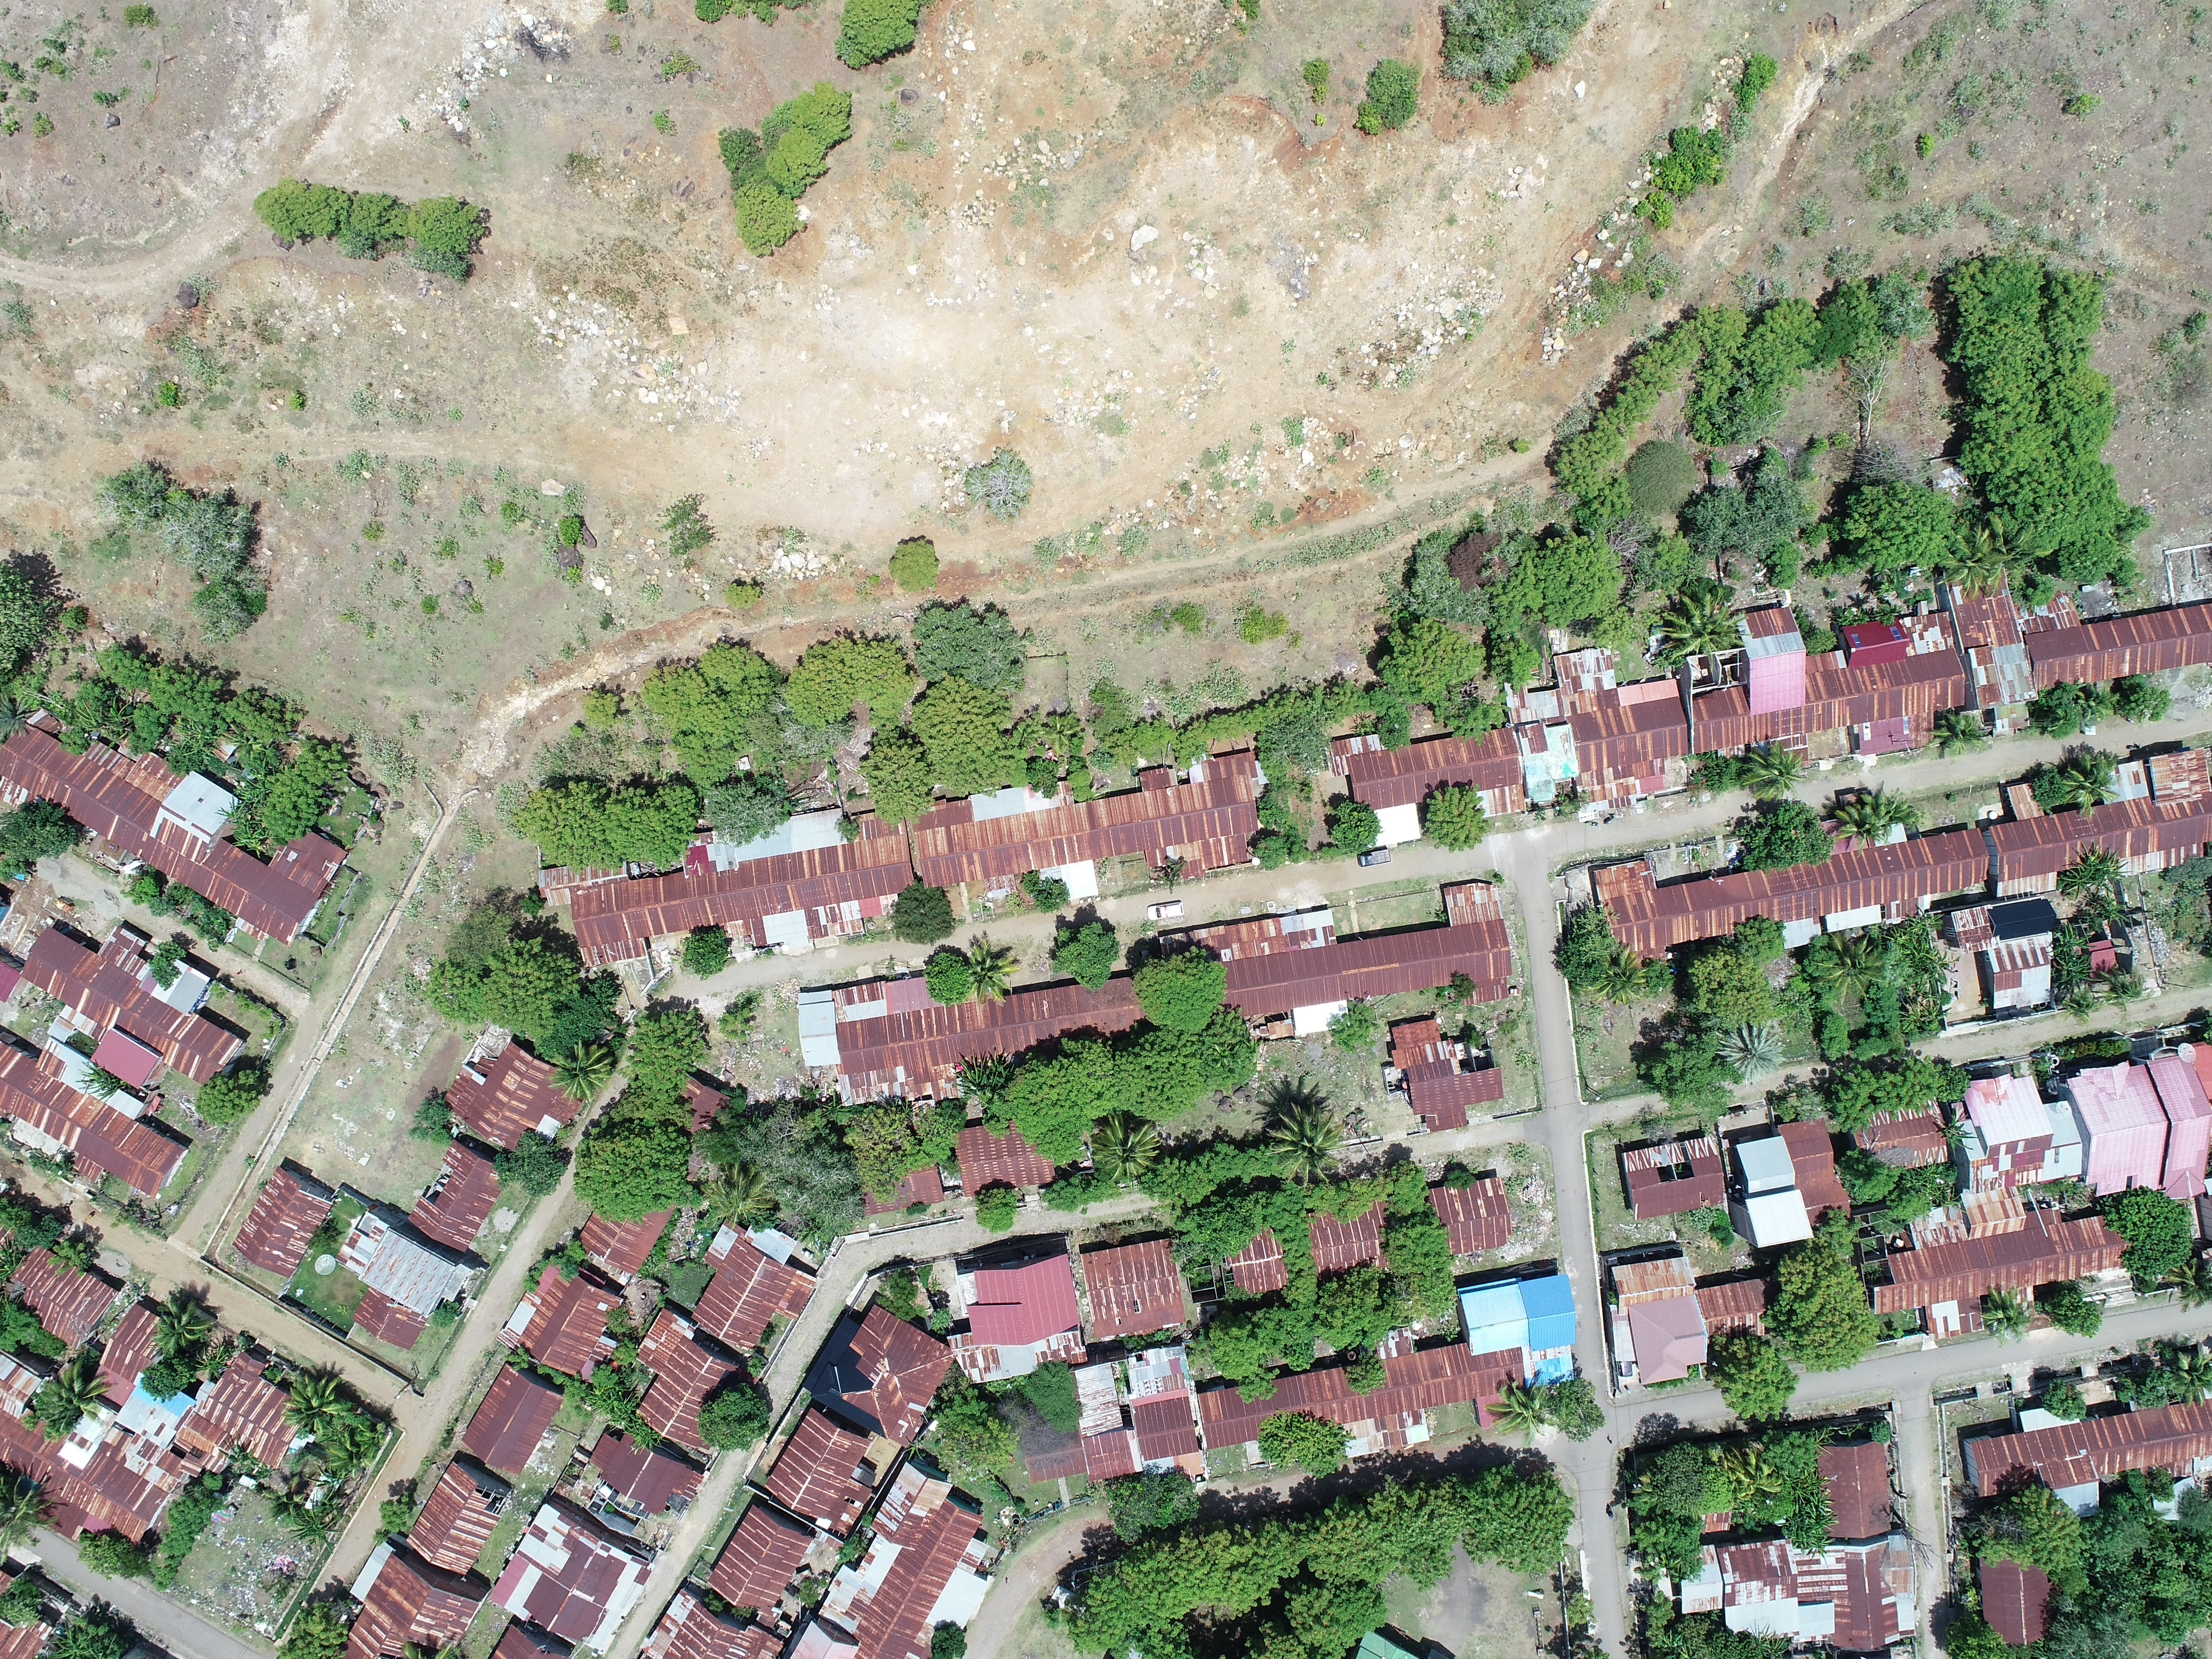
\includegraphics [width = 11.5cm,]{image/DJI_0880}}
	\caption{Sampel foto Udara 2}
	\label{Sampel foto Udara 2} % cuman gambar dummy ya !
\end{figure}
\begin{figure}[H]
        \centering
	\frame{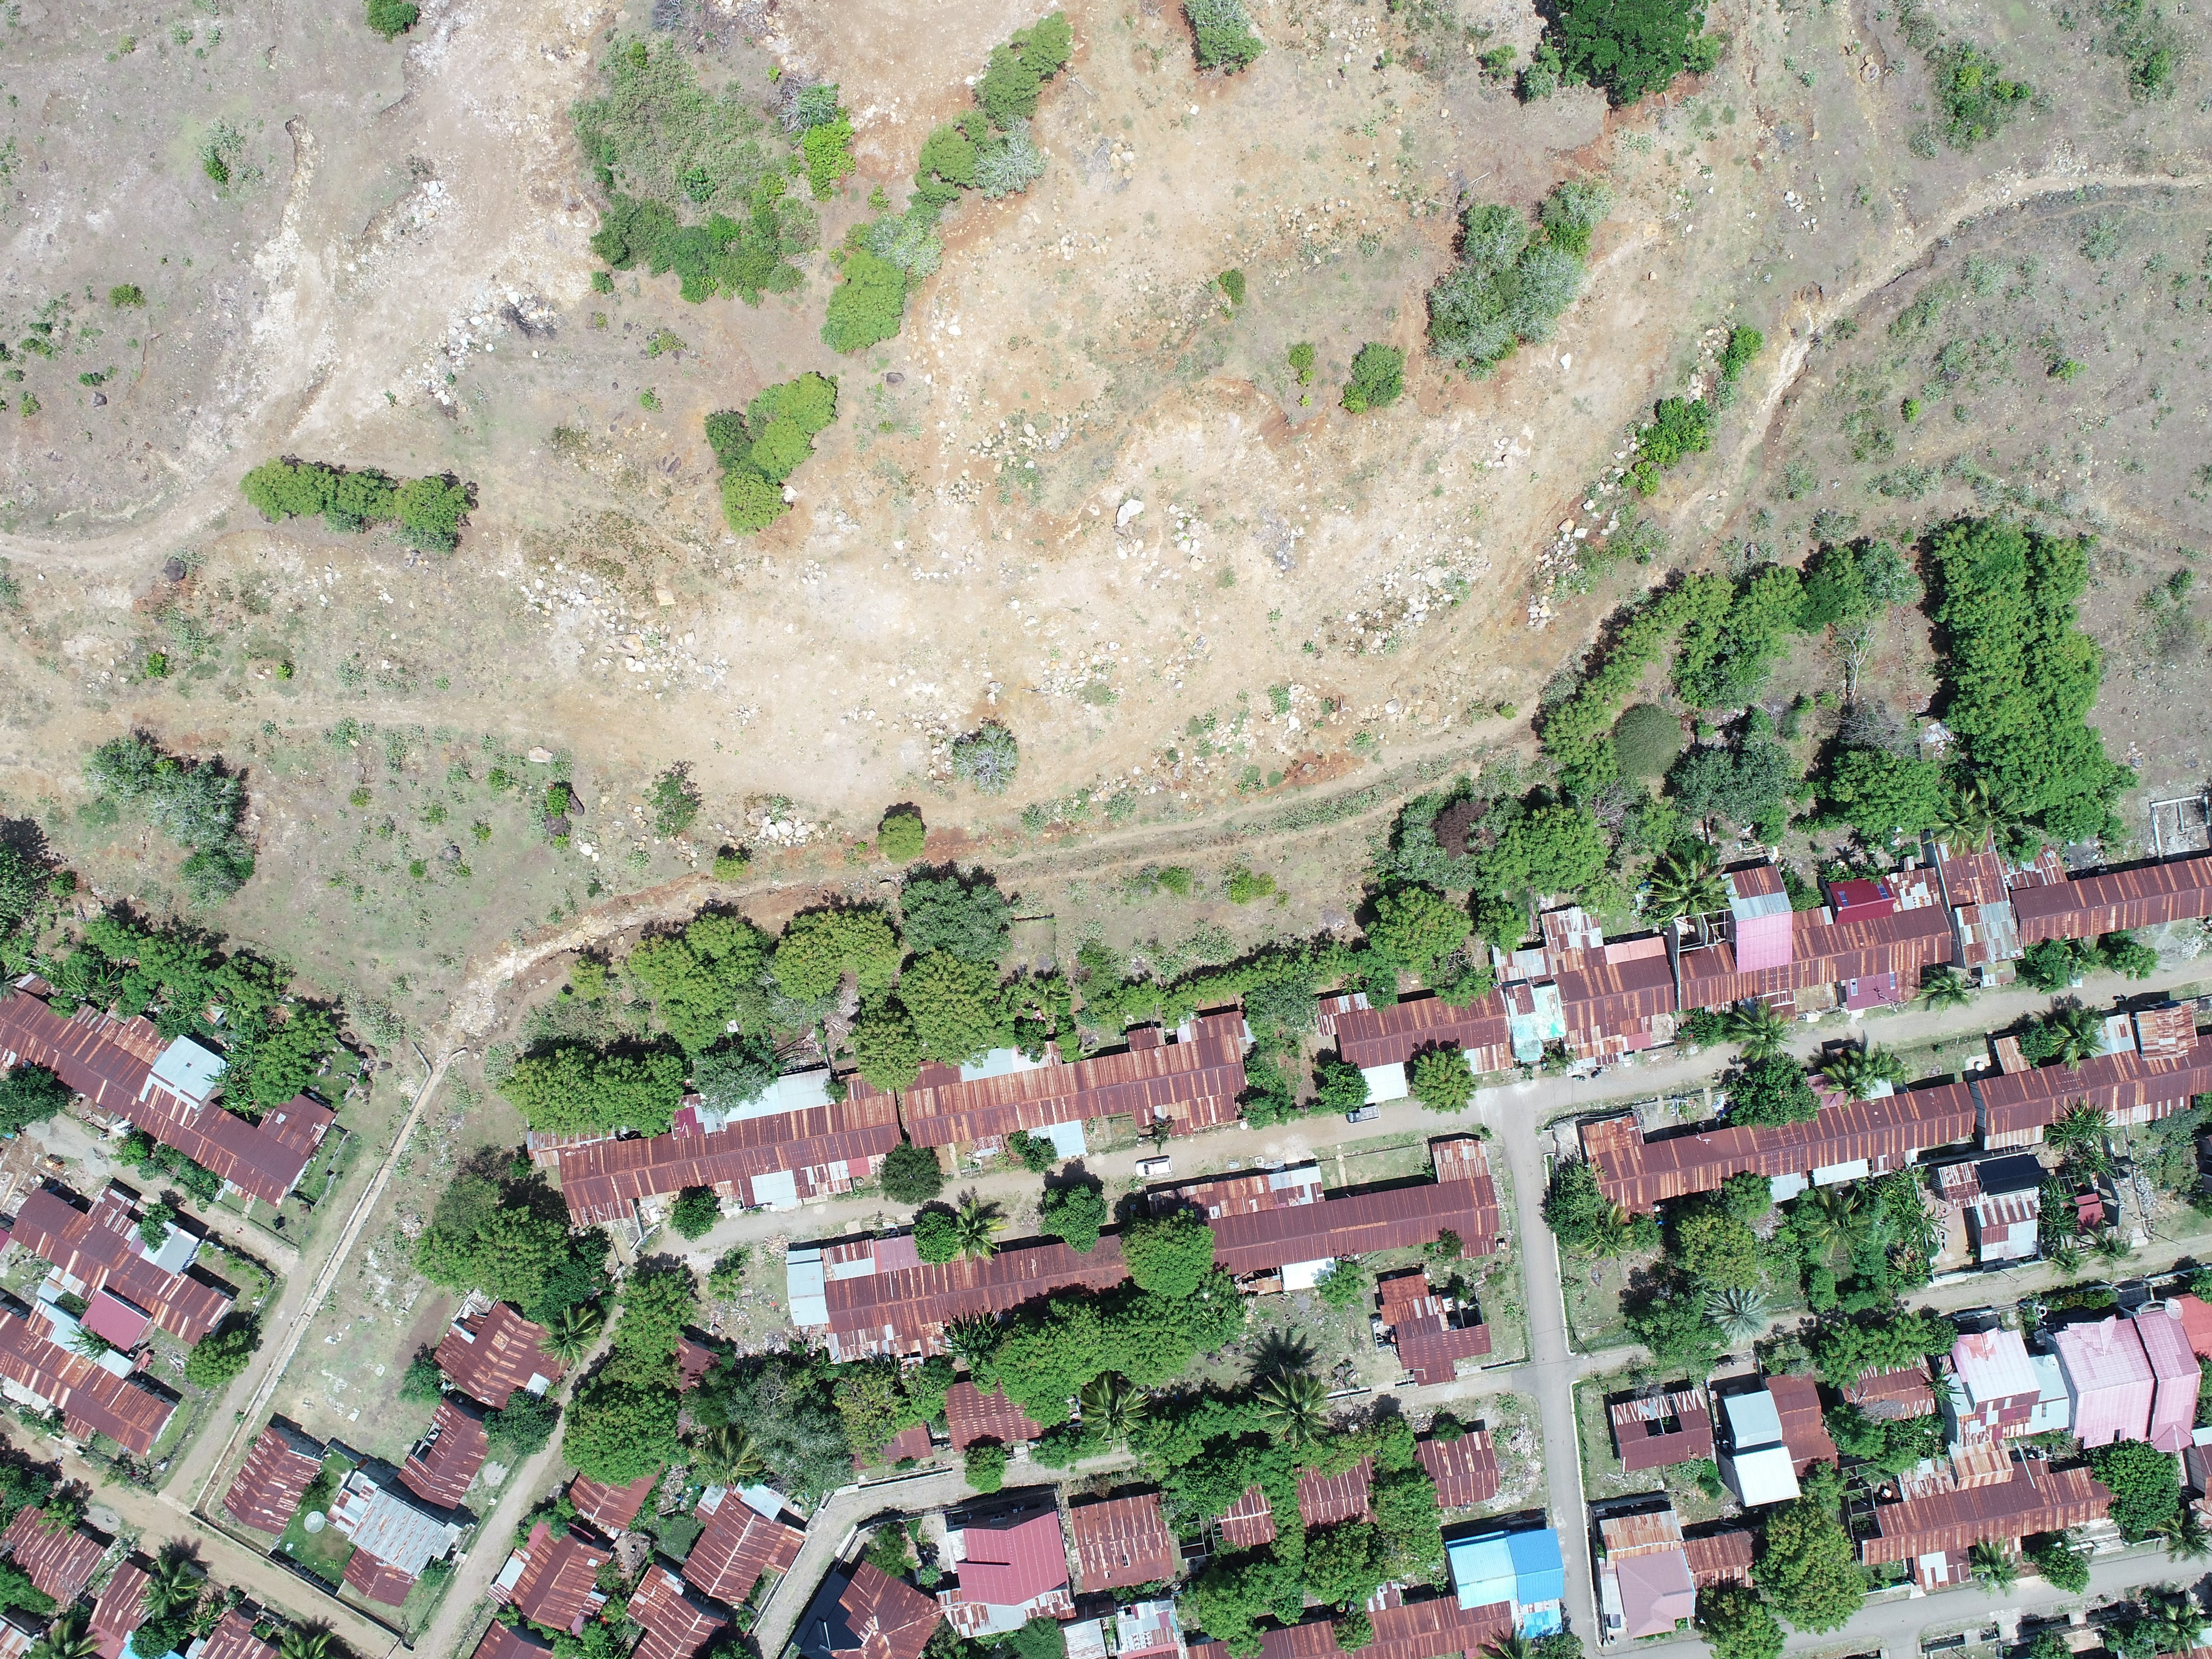
\includegraphics [width = 11.5cm,]{image/DJI_0881}}
	\caption{Sampel foto Udara 3}
	\label{Sampel foto Udara 3} % cuman gambar dummy ya !
\end{figure}

\section{Metode Penelitian}

Analisis akuisisi data dan mosaik citra resolusi tinggi kawasan kampus II Universitas Syiah Kuala di Kecamatan Mesjid Raya, Aceh Besar dilakukan dengan beberapa tahapan, Gambar \ref{alur} dibawah ini memberikan informasi mengenai tahapan tersebut.

\begin{figure}[H]
	\centering
	{\includegraphics [width = 11.5cm,]{image/blank diagram.png}}
	\caption{Diagram alur penelitian}
	\label{alur} % cuman gambar dummy ya !
\end{figure}

\subsection{Studi Literatur}
Studi literatur dilakukan untuk memberikan dasar teoritis dan kontekstual bagi penelitian yang akan dilaksanakan. Proses ini melibatkan tinjauan yang mendalam terhadap kajian-kajian sebelumnya, jurnal ilmiah, buku, dan sumber-sumber lain yang relevan dengan topik penelitian. Analisis literatur membantu peneliti untuk memahami kemajuan pengetahuan terbaru, menganalisis pendekatan-pendekatan yang telah diambil oleh peneliti sebelumnya, serta mengidentifikasi kebutuhan solusi yang masih perlu dikembangkan. Analisis literatur juga membantu dalam menghindari duplikasi penelitian dan memastikan kontribusi penelitian baru terhadap literatur yang sudah ada.

\subsection{Analisis Akuisisi Data}
Akuisisi data citra di kawasan Kampus USK II, Kecamatan Mesjid Raya, Aceh Besar, dilakukan dengan menggunakan \textit{drone} DJI Phantom 4 Pro. Proses ini dimulai dengan perencanaan penerbangan \textit{drone} yang matang, meliputi penentuan area yang akan dipetakan, jalur penerbangan yang efisien, ketinggian terbang yang optimal, dan pengaturan \textit{overlap} antar citra yang diambil. Tahap selanjutnya adalah pengaturan kamera dan sensor yang terpasang pada \textit{drone} agar dapat menghasilkan kualitas citra yang baik, seperti resolusi gambar, laju pengambilan gambar, dan kemampuan sensor untuk menangkap informasi yang dibutuhkan. Pada tahap berikutnya, \textit{drone} melakukan penerbangan sesuai jalur yang telah direncanakan dan mengambil citra secara berangsur-angsur, merata, dan menyeluruh untuk mencakup seluruh kawasan lahan Kampus USK II. Proses ini membutuhkan ketelitian dan pemantauan yang cermat untuk memastikan tidak ada area yang terlewatkan dan tidak ada gangguan eksternal yang dapat mempengaruhi kualitas data. Setelah citra berhasil diambil, data tersebut ditransmisikan media penyimpanan yang sesuai dengan hati-hati untuk menghindari kehilangan atau kerusakan data. Setelah data berhasil disimpan, dilakukan verifikasi dan kontrol kualitas data yang meliputi pemeriksaan kelengkapan data, konsistensi resolusi dan kualitas citra, serta identifikasi adanya kesalahan atau noise yang dapat mempengaruhi analisis data. Langkah ini penting untuk memastikan bahwa data yang diperoleh memenuhi standar yang dibutuhkan untuk keperluan analisis selanjutnya. Analisis akuisisi data yang cermat dan terencana akan memastikan data citra yang diperoleh dari kawasan Kampus USK II memiliki kualitas yang baik dan dapat digunakan untuk berbagai keperluan, seperti pemantauan lingkungan, perencanaan infrastruktur, atau analisis tutupan lahan dan penggunaan lahan.

\subsection{Pengumpulan Data}
Dalam penelitian ini, proses pengumpulan data telah selesai dilaksanakan, dan penulis kini fokus pada pengorganisasian data ke dalam struktur folder yang sistematis untuk memudahkan analisis dan pemrosesan selanjutnya. Data yang diatur mencakup dua kategori utama yaitu serangkaian gambar hasil pemotretan menggunakan \textit{drone} dan data referensi lapangan berupa koordinat Ground Control Points (GCP) yang disimpan dalam format file teks. Citra-citra drone akan menjadi input utama dalam proses mosaik, sementara data GCP berperan krusial dalam meningkatkan akurasi geometrik dan georeferensi dari citra mosaik yang akan dihasilkan. Pengaturan data yang terstruktur ini tidak hanya akan memperlancar alur kerja pengolahan citra, tetapi juga akan mempermudah proses validasi  dan analisis akurasi spasial dari \textit{orthomosaic} yang dihasilkan. Selain itu, organisasi data yang baik akan memungkinkan perbandingan yang lebih efisien antara hasil pengolahan menggunakan Agisoft Metashape dan Pix4Dmapper, sesuai dengan tujuan penelitian untuk membandingkan kinerja kedua perangkat lunak tersebut.

\subsection{Mosaik}

Setelah berhasil mengumpulkan data citra dari seluruh wilayah penelitian di lahan Kampus 
USK II, langkah berikutnya adalah melakukan proses mosaik pada keseluruhan 
gambar. Hal ini bertujuan untuk menciptakan representasi visual menyeluruh dari 
kawasan yang telah diamati. Dalam penelitian ini, penulis melakukan proses mosaik 
pada citra menggunakan dua perangkat lunak berbeda, yakni Agisoft metashape dan PIX4Dmapper. 
Tujuan dari pendekatan ganda ini adalah untuk membandingkan hasil mosaik dari 
kedua perangkat lunak tersebut dan kemudian menyimpulkan manakah yang 
memberikan hasil yang lebih baik dan optimal dalam melakukan proses mosaik.

\subsection{Analisis Perbandingan}

\par Dalam penelitian ini, analisis komparatif berfokus pada tiga aspek utama yang dihasilkan oleh dua perangkat lunak fotogrametri, Agisoft Metashape dan Pix4Dmapper: akurasi geografis, resolusi spasial, dan efisiensi waktu pemrosesan. Evaluasi dilakukan dengan mempertimbangkan ground resolution dan resolusi orthomosaic yang dihasilkan oleh kedua perangkat lunak tersebut. Untuk menilai keakuratan geografis, akan dilakukan perbandingan menggunakan beberapa matriks evaluasi, termasuk \textit{Circular Error, Linear Error, dan Root Mean Square Error} (RMSE). Selain itu, penelitian ini akan mengukur dan membandingkan waktu yang dibutuhkan oleh masing-masing perangkat lunak untuk menyelesaikan proses pengolahan data. Terakhir, studi ini akan memverifikasi apakah hasil dari kedua perangkat lunak tersebut memenuhi standar ketelitian yang ditetapkan untuk peta Rupa Bumi Indonesia (RBI).


%-----------------------------------------------------------------------------%

% Baris ini digunakan untuk membantu dalam melakukan sitasi
% Karena diapit dengan comment, maka baris ini akan diabaikan
% oleh compiler LaTeX.
\begin{comment}
\bibliography{daftar-pustaka}
\end{comment}